\documentclass[conference]{IEEEtran}
\IEEEoverridecommandlockouts
% The preceding line is only needed to identify funding in the first footnote. If that is unneeded, please comment it out.
\usepackage{cite}
\usepackage{amsmath,amssymb,amsfonts}
\usepackage{algorithmic}
\usepackage{graphicx}
\usepackage{dblfloatfix}

\def\BibTeX{{\rm B\kern-.05em{\sc i\kern-.025em b}\kern-.08em
    T\kern-.1667em\lower.7ex\hbox{E}\kern-.125emX}}
\begin{document}

\title{Asymmetric Gaussian Mixtures with Reversible Jump MCMC\\
%{\footnotesize \textsuperscript{*}Note: Sub-titles are not captured in Xplore and
%should not be used}
%\thanks{Identify applicable funding agency here. If none, delete this.}
}

\author{\IEEEauthorblockN{Shuai Fu}
\IEEEauthorblockA{\textit{Faculty of Engineering and Computer Science}\\
\textit{Concordia University}\\
Montreal, Canada\\
f\_shuai@encs.concordia.ca}
\and
\IEEEauthorblockN{Nizar Bouguila}
\IEEEauthorblockA{\textit{Concordia Institute for Information Systems Engineering} \\
\textit{Concordia University}\\
Montreal, Canada \\
bouguila@ciise.concordia.ca}
}

\maketitle

\begin{abstract}
We propose a fully Bayesian learning approach using reversible jump Markov  chain Monte Carlo (RJMCMC) for asymmetric Gaussian mixtures (AGM). Compared to classic Gaussian mixture model, AGM doesn't imply that target data is symmetric which brings flexibility and better fitting results. This paper also introduces a RJMCMC learning implementation based on Metropolis-Hastings (MH) within Gibbs sampling method. As an improvement of traditional sampling-based MCMC learning, RJMCMC has no assumption concerning the number of components and, therefore, the AGM model itself could be transferred between iterations. For better evaluating models with different mixture components number, the model selection is achieved by calculating integrated likelihood using Laplace approximation to figure out the best-fit components number. We selected both synthetic and a challenging spam filtering datasets to show the merits of the proposed model. 
\end{abstract}

\begin{IEEEkeywords}
Asymmetric Gaussian Mixture, Metropolis-Hastings, Gibbs sampling, RJMCMC, Laplace approximation, Spam Filtering
\end{IEEEkeywords}

\section{Introduction}
Statistics reveal a crucial fact that more than 59\% of worldwide e-mail traffic is considered as unsolicited messages, also well known as spams, in 2017 \cite{spamStats}. Most spams are irritating and resource-consuming, and some of them are extremely dangerous in terms of phishing scam, fee fraud, job offer scam, etc,. Since the damages of spam are persistent and significant not only for individuals but also for governments, companies and organizations, many spam filtering technologies have been proposed to address this issue and eliminate unwanted e-mails automatically over recent decades. 

Most modern machine learning-based filtering approaches can be classified into two categories: supervised and unsupervised. As an important solution for spam filtering, Supervised approaches\cite{supervisedSpam} perform well under some circumstances, but compared to unsupervised learning methods, they have significant limitations and drawbacks because supervised classifiers cannot identify new spam patterns not presented in their training datasets. Once new patterns are discovered, model adjustment will be needed. Furthermore, poor training datasets could cause inductive bias and overfitting problems which will affect the accuracy of the models. Therefore, unsupervised solution has been increasingly drawing attention because of its flexibility and robustness.

As widely deployed unsupervised learning approaches, mixture models can be viewed as an improvement of independent methodologies which superimposes a finite number of components while respecting the dependency between data clusters, demonstrating outstanding suitability and generality especially for complex high-dimensional datasets. More precisely, for Gaussian-like datasets, Gaussian mixture model (GMM) \cite{b1} is proven as an effective   learning approach in several domains such as computer vision, pattern recognition and data mining. In this paper, we show the merits of asymmetric Gaussian mixture (AGM) model \cite{b2} for clustering because of its two variance parameters for left and right parts of each distribution in the mixture which brings more accuracy of fitting real datasets which could be asymmetric or even non-Gaussian. 

Estimating the parameters of mixture models could be a challenging task. The maximum-likelihood-based expectation maximization (EM) \cite{b3} algorithm is one of the most popular parameter learning approaches. However, the disadvantages of EM algorithm are also obvious. Given the fact that EM approximates values of mixture parameters in a deterministic way this could cause slow convergence and compromise the usability of the algorithm. Furthermore, bad initialization and overfitting problems\cite{b4} \cite{b5} will also significantly affect its accuracy. Therefore, fully Bayesian learning algorithms, such as Markov Chain Monte Carlo (MCMC) based implementations, are found to be useful to eliminate overfitting problems in mixture parameter learning by introducing prior and posterior distributions for mixture parameters. In this paper, the learning process is accomplished by a hybrid MCMC algorithm, which is well known as Metropolis-Hastings within Gibbs sampling\cite{b4}, based on both Metropolis-Hastings (Hastings, 1970)\cite{b6} and Gibbs sampling (Geman and Geman, 1984)\cite{b7} methods because the main difficulty of classic MCMC method is that, under some circumstances, direct sampling is not always straightforward. Moreover, we reinforce the learning algorithm by introducing reversible jump MCMC (RJMCMC)\cite{b5} methodology to increase the flexibility of AGM model by allowing model transfer throughout iterations via increasing (component birth/split step) and decreasing (component death/merge step) mixture components. Because of the stochastic sampling-based learning process, learning iterations could end up with different number of components so we choose marginal likelihood\cite{b4} to perform model selection in order to evaluate fitting results between models.

The rest of this paper is organized as follows. In the next Section, we present our Bayesian model. Section III is devoted to the experimental results. Section IV concludes the paper.


\section{Bayesian model}
\subsection{Asymmetric Gaussian Mixture Model}
The likelihood function of AGM model\cite{b2} with $M$ mixture components can be defined as follows:

\begin{align}
p(\mathcal{X}|\Theta) = \prod_{i=i}^N \sum_{j=1}^Mp_jp(X_i|\xi_j)
\label{eq:likelihood}
\end{align}

where $\mathcal{X} = (X_1,...,X_N)$ reprensents the dataset with $N$ observations, $\Theta = \{p_1,...,p_M, \xi_1,...,\xi_M\}$ defines the mxiture parameters set of AGM mixture model including component weight $p_j$ (0 $< p_j \leq$ 1 and $\sum_{j=1}^Mp_j$ = 1) and asymmetric Gaussian distribution (AGD) parameters set $\xi_j$ for mixture component $j$. Assuming the dataset $\mathcal{X}$ is $d$-dimensional, for each observation $X_n = (x_{n1},...,x_{nd})\in\mathcal{X}$, the probability density function\cite{b2} for $j$-th component of the model can be defined as follows:

\begin{multline}
p(X_n|\xi_j) \propto \prod_{k=1}^{d} \frac{1}{(\sigma_{l_{jk}}+\sigma_{r_{jk}})} \\
\times \left\{\begin{matrix}
\exp \begin{bmatrix}
-\frac{(x_{nk}-\mu_{jk})^2}{2(\sigma_{l_{jk}})^2}
\end{bmatrix}\ if\ x_{nk}\ <\ \mu_{jk} \\ 
\exp \begin{bmatrix}
-\frac{(x_{nk}-\mu_{jk})^2}{2(\sigma_{r_{jk}})^2}
\end{bmatrix}\ if\ x_{nk}\ \geqslant\ \mu_{jk} \\ 
\end{matrix}\right.
\label{eq:pdf}
\end{multline}

parameters set of component $j$ is $\xi_j = (\mu_j,\sigma_{lj},\sigma_{rj})$ where $\mu_j = (\mu_{j1},...,\mu_{jd})$ is the mean, $\sigma_{lj} = (\sigma_{lj1},...,\sigma_{ljd})$ and $\sigma_{rj} = (\sigma_{rj1},...,\sigma_{rjd})$ are the left and right standard deviation vectors of AGD . 

We introduce a $M$-dimensional membership vector $Z$ for each observation $X_i\in\mathcal{X}, Z_i = (Z_{i1},...,Z_{iM})$ which indicates to which specific component $X_i$ belongs\cite{b8}, such that:
\begin{align}
Z_{ij} = \left\{\begin{matrix}
1\qquad\mbox{ if }X_i\mbox{  belongs to component }j \\
0\qquad\quad\qquad \mbox{otherwise} \qquad\qquad\quad\quad \\
\end{matrix}\right.
\label{eq:memVector}
\end{align}
in other words, $Z_{ij} = 1$ only if observation $X_i$ has the highest probability of belonging to component $j$ and accordingly, for other components, $Z_{ij} = 0$. 

Therefore, the complete likelihood function can be derived by combining Eq. \eqref{eq:likelihood} and Eq. \eqref{eq:memVector} as follows:
\begin{align}
p(\mathcal{X}, Z|\Theta) = \prod_{i=1}^{N}\prod_{j=1}^{M}(p_jp(X_i|\xi_j))^{Z_{ij}}
\label{eq:compPdf}
\end{align}

\subsection{Priors and Posteriors}
As discussed before, MH-within-Gibbs based RJMCMC learning algorithm implementation defines priors and posteriors for mixture weighs and parameters to avoid direct sampling. For a specific iteration $t$, since mixture weight $p_j$ satisfies 0 $< p_j \leq$ 1 and $\sum_{j=1}^Mp_j$ = 1, a nature choice of the prior is Dirichlet distribution\cite{b10} as follows:
\begin{align}
\pi(p_j^{(t)}) \sim \mathcal{D}(\gamma_1,...,\gamma_M )
\label{eq:priorWeight}
\end{align}

where $\gamma_j$ is known hyperparameter. By considering the membership vector Z as a condition, The posterior probability of mixture weight $p_j$ is defined as follows:
\begin{align}
p(p_j^{(t)}|Z^{(t)}) \sim \mathcal{D}(\gamma_1 + n_1^{(t)},...,\gamma_M + n_M^{(t)})
\label{eq:posterWeight}
\end{align}

where $n_j$ represents number of observations belonging to component $j$ which could be calculated using membership vectors as follows:
\begin{align}
n_j^{(t)} = \sum_{i=1}^NZ_{ij}\ (j = 1,...,M) 
\label{eq:nj}
\end{align}

The same idea applies to the sampling process of mixture parameters. The proposal posterior distribution is  $\xi^{(t)} \sim q(\xi|\xi^{(t-1)})$. To be more specific, for parameters of AGM model $\xi^{(t)} = (\mu^{(t)}, \sigma_{l}^{(t)}, \sigma_{r}^{(t)})$, we choose $d$-dimensional Gaussian distributions as posterior distributions respectively:
\begin{align}
\mu_j^{(t)} \sim \mathcal{N}_d(\mu_j^{(t-1)},\Sigma),
\sigma_{lj}^{(t)} \sim \mathcal{N}_d(\sigma_{lj}^{(t-1)},\Sigma),
\sigma_{rj}^{(t)} \sim \mathcal{N}_d(\sigma_{rj}^{(t-1)},\Sigma)
\label{eq:posters}
\end{align}

where $\Sigma$ is $d$ x $d$ identity matrix which makes the sampling a random walk MCMC process. Correspondingly, the priors are $\mu \sim \mathcal{N}_d(\eta,\Sigma)$ and $\sigma_l, \sigma_r \sim \mathcal{N}_d(\tau,\Sigma)$ given known hyperparameters $\eta$ and $\tau$.

\subsection{Learning Algorithm}
\subsubsection*{MH-within-Gibbs}
As a sampling-based learning algorithm, MH-within-Gibbs method performs random sampling from posteriors of parameters, and then calculate the acceptance ratio $r$ in order to make a decision whether the new samples should be accepted or discarded for next iteration. Because of the usage of membership vector $Z$, the mixture weight $p_j$ can be derived within Gibbs sampling part. Therefore, it will be excluded from the calculation of the acceptance ratio $r$ which is defined as follows:
\begin{align}
r = \frac{p(\mathcal{X}|\Theta^{(t)})\pi(\Theta^{(t)})q(\Theta^{(t-1)}|\Theta^{(t)})}{p(\mathcal{X}|\Theta^{(t-1)})\pi(\Theta^{(t-1)})q(\Theta^{(t)}|\Theta^{(t-1)})}
\label{eq:r}
\end{align}

Once acceptance ratio $r$ is derived, we compute acceptance probability $\alpha = min[1,r]$ \cite{b11}. Then $u \sim U_{[0,1]}$ is supposed to be generated randomly. If $\alpha < u$, the proposed move should be accepted and parameters should be updated by $p^{(t)}$ and $\xi^{(t)}$ for next iteration. Otherwise, we discard $p^{(t)}$, $\xi^{(t)}$ and set $p^{(t)} = p^{(t-1)}$, $\xi^{(t)} = \xi^{(t-1)}$. 
\bigskip

\subsubsection*{RJMCMC moves}
Traditional MH-within-Gibbs algorithm assumes that the components number $M$ is given and persistent throughout the learning process. However, because of bad initialization or just leaking of information, components number $M$ could be inaccurate or unknown. Under these circumstances, RJMCMC algorithm is found to be useful by providing extra four independent steps (birth/split steps and death/merge steps) into learning process which could change components number $M$, therefore, brings more generalities.

Letting $M_{min}$ and $M_{max}$ denote the minimum and maximum number of components $M$, assuming the probabilities of performing birth/split and death/merge steps are $b_m$ and $d_m = 1 - b_m$ for $m = M_{min},\dots,M_{max}$ respectively. Obviously, $b_{M_{max}}=0$ and $d_{M_{min}}=0$. Correspondingly, $d_{M_{max}}=1-b_{M_{max}} = 1$ and $b_{M_{min}}=1-d_{M_{min}}=1$. For $m=M_{min}+1,\dots,M_{max}-1$, due to simplification reasons, we choose the same value for both $b_m$ and $d_m$ as $b_m=d_m=0.5$. Within every iteration, we generate a random value $u' \sim U_{[0,1]}$ respectively for the four RJMCMC steps. If $b_m >= u'$ or $d_m >= u'$, birth/split or death/merge steps should be performed correspondingly.\cite{b1}

\textbf{Merge and Split Steps}: Randomly choose two components $(j_1,j_2)$ satisfying that $\mu_{j_1}<\mu_{j_2}$ with no other $\mu_j$ in the interval $[\mu_{j_1},\mu_{j_2}]$. The newly merged component $j'$ will contain the observations that previously belong to both component $j_1$ and $j_2$. At the meanwhile, reduce current value of components number $m=m-1$, then calculate mixture weight and parameters for $j'$ as follows:
\begin{multline}
\qquad\qquad\qquad\qquad p_{j'} = p_{j_1}+p_{j_2} \\
p_{j'}\mu_{j'} = p_{j_1}\mu_{j_1} + p_{j_2}\mu_{j_2} \\
p_{j'}(\mu_{j'}^2 + \sigma_{j'l}^2) = p_{j_1}(\mu_{j_1}^2 + \sigma_{j_1l}^2)+p_{j_1}(\mu_{j_1}^2 + \sigma_{j_1l}^2) \qquad \\
p_{j'}(\mu_{j'}^2 + \sigma_{j'r}^2) = p_{j_1}(\mu_{j_1}^2 + \sigma_{j_1r}^2)+p_{j_1}(\mu_{j_1}^2 + \sigma_{j_1r}^2)
\label{eq:merge}
\end{multline}

As a reverse of merge step, we split component $j'$ into two ($j_1$ and $j_2$) with 3 degrees of freedom $(u_1 \sim Beta(2,2), u_2 \sim Beta(2,2), u_3 \sim Beta(1,1))$ and, accordingly, increase $m=m+1$. Therefore, mixture parameters for split components can be calculated as follows:
\begin{multline}
\qquad\qquad\qquad p_{j_1} = p_{j'}u_1, p_{j_2} = p_{j'}u_2 \\
\mu_{j_1} = \mu_{j'} - \frac{u_2(\sigma_{j'l}+\sigma_{j'r})}{2} \sqrt{\frac{p_{j_2}}{p_{j_1}}} \\
\mu_{j_2} = \mu_{j'} + \frac{u_2(\sigma_{j'l}+\sigma_{j'r})}{2} \sqrt{\frac{p_{j_1}}{p_{j_2}}} \\
\sigma_{j_1l}^2 = u_3(1-u_2^2)\sigma_{j'l}^2\frac{p_{j'}}{p_{j_1}} \\
\sigma_{j_1r}^2 = u_3(1-u_2^2)\sigma_{j'r}^2\frac{p_{j'}}{p_{j_1}} \\
\sigma_{j_2l}^2 = (1-u_3)(1-u_2^2)\sigma_{j'l}^2\frac{p_{j'}}{p_{j_2}} \\
\sigma_{j_2r}^2 = (1-u_3)(1-u_2^2)\sigma_{j'r}^2\frac{p_{j'}}{p_{j_2}} \qquad\quad
\label{eq:split}
\end{multline}

In order to decide whether the merge and split steps should be accepted or not, we calculate the acceptance probability $\mathcal{A}$ which is described in\cite{b1}. Therefore, the acceptance probability for merge step is $\min(1,\mathcal{A})$ and, correspondingly, for split step is $\min(1,\mathcal{A}^{-1})$.

\textbf{Birth and Death Steps}: Compared to merge and split steps, birth and death steps are relatively straightforward because the newborn and dead components are empty ones which means parameter re-calculation is not needed. Mixture weight $p_{new}$ in birth step can be obtained by sampling from Beat distribution $p_{new} \sim Beta(1,m)$ and mixture parameters can be derived from the priors as follows\cite{casella}:
\begin{align}
\mu \sim \mathcal{N}(\xi,\kappa^{-1}), \quad \sigma_{l}^{-2},\sigma_{r}^{-2} \sim \Gamma(\alpha,\beta), \quad \beta \sim \Gamma(g,h)
\label{eq:prior}
\end{align}
where hyperparameters $\kappa$, $\alpha$, $g$ and $h$ are estimated by data and $\xi$ is the midpoint of the observations. For death step, a random choice is made between existing empty components and simply delete the selected one. If there is no empty component, death step will be skipped. After birth and death steps, mixture weights $p_j$ should be re-scaled so that all weights sum to 1. Acceptance probability $\mathcal{A}'$ for birth and death steps is also required as the one for merge and split steps. The probabilities of occurrence of birth and death steps are $\min(1,\mathcal{A}')$ and $\min(1,\mathcal{A}'^{-1})$\cite{b1}.

Finally, a typical reversible jump MH-within-Gibbs learning procedure for AGM model can be summarized as follows:
\bigskip

\noindent\textbf{Input:} Data observations $\mathcal{X}$ and components number $M$ \\
\textbf{Output:} AGM mixture parameter set $\Theta$
\begin{enumerate}
\item Initialization
\item Step $t$: For $t = 1,\ldots$
\begin{enumerate}
\item[]\textbf{Gibbs sampling part}
\item Generate $Z^{(t)}$ from Eq. \eqref{eq:memVector}
\item Compute $n_j^{(t)}$ from Eq. \eqref{eq:nj}
\item Generate $p_j^{(t)}$ from Eq. \eqref{eq:posterWeight}
\item[] \textbf{Metropolis-Hastings part}
\item Sample $\xi_j^{(t)}$ ($\mu_j^{(t)}, \sigma_{lj}^{(t)}, \sigma_{rj}^{(t)}$) from Eqs. \eqref{eq:posters}
\item Compute acceptance ratio $r$ from Eq. \eqref{eq:r}
\item Generate $\alpha = min[1,r]$ and $u \sim U_{[0,1]}$
\item If $\alpha \geq u$ then $\xi^{(t)} = \xi^{(t-1)}$
\item[] \textbf{RJMCMC part}
\item Generate $u' \sim U_{[0,1]}$. If $b_m>=u'$, perform split or birth step, then calculate acceptance probability $\mathcal{A}$. If the step is accepted, set $m=m+1$.
\item Generate $u' \sim U_{[0,1]}$. If $d_m>=u'$, perform merge or death step, then calculate acceptance probability $\mathcal{A}'$. If the step is accepted, set $m=m-1$.
\end{enumerate}
\end{enumerate}

\section{Experimental results}
\begin{figure}[b]
\centering
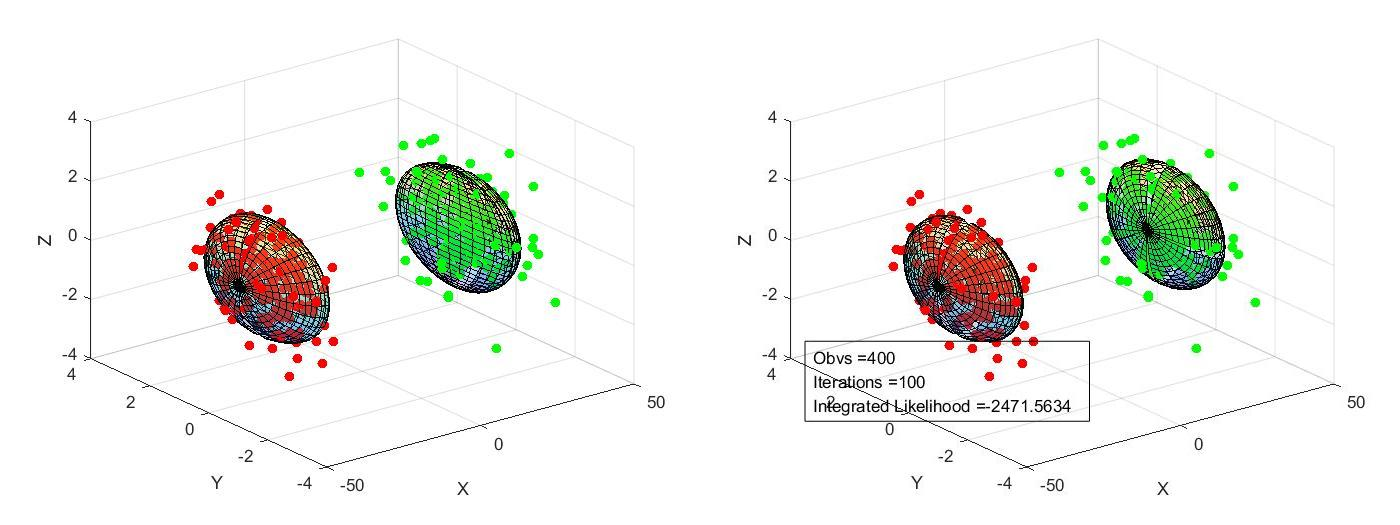
\includegraphics[width=0.45\paperwidth]{syn.jpg}
\caption{Original synthetic data grouping and learning results}
\label{fig:1}
\end{figure}


\subsection{Synthetic Data}

We start by testing the performance of our model on a 3-D synthetic dataset with 400 observations composed of clusters. Hyperparameters related to the calculations of mixture weights and parameters are set as $\gamma_j = 1$ and both $\eta$ and $\tau$ are considered as $d$-dimensional zero vectors. Consequently, hyperparameters for priors of mixture parameters are set as follows\cite{b13}:
\begin{align}
\kappa = \frac{1}{\mathcal{R}^2}, \quad \alpha = 3, \quad g=0.3, \quad h=\frac{100g}{\alpha\mathcal{R}^2}
\label{eq:hypers}
\end{align}
where $\mathcal{R}$ is the interval of variation of observations.

Figure \ref{fig:1} compares original grouping and RJMCMC learning results. Euclidean distances between means of original and estimated clusters are 1.7496 and 1.6263 and standard deviations for $\sigma_l$ and $\sigma_r$ are [0.60272,1.3511] and [1.3209,0.78647], demonstrating a promising accuracy of AGM model.

\subsection{Spam Filtering}

\begin{table}[b]
\caption{AGM Statistics}
\begin{center}
\begin{tabular}{|c|c|c|}
\hline
\multicolumn{1}{|p{2cm}|}{\centering \textbf{Init. Comp. Number $m$}} & \multicolumn{1}{|p{2cm}|}{\centering \textbf{\textit{Accuracy}}} & \multicolumn{1}{|p{2cm}|}{\centering \textbf{\textit{Integrated Likelihood}}}\\
\hline
$m=1$ & 55.64\% & $5.7074\mathrm{e}{5}$\\
$m=2$ & 51.21\% & $4.0543\mathrm{e}{5}$ \\
$m=3$ & 58.99\% & $8.4238\mathrm{e}{5}$ \\
\hline
\end{tabular}
\label{tab1}
\end{center}
\end{table}

\begin{table}[b]
\caption{Confusion Matrices and Statistics of GMM and AGM}
\begin{center}

\begin{minipage}{0.75\textwidth}
\begin{flushleft}
\begin{tabular}{cc}

\begin{minipage}{.3\textwidth} 
\begin{center}
\textbf{GMM} \\
\begin{tabular}{|c|c|c|}
\hline
 & \multicolumn{1}{|p{.7cm}|}{\centering \textbf{\textit{NF $^{\mathrm{a}}$}}} & \multicolumn{1}{|p{.7cm}|}{\centering \textbf{\textit{F $^{\mathrm{b}}$}}}\\
\hline
\multicolumn{1}{|p{.7cm}|}{\centering \textbf{\textit{NF}}} & 35 & 1778\\
\multicolumn{1}{|p{.7cm}|}{\centering \textbf{\textit{F}}} & 295 & 2493\\
\hline
\end{tabular}
\end{center}
\end{minipage} &

\begin{minipage}{.3\textwidth}    
\begin{center}
\textbf{AGM} \\
\begin{tabular}{|c|c|c|}
\hline
 & \multicolumn{1}{|p{.7cm}|}{\centering \textbf{\textit{NF}}} & \multicolumn{1}{|p{.7cm}|}{\centering \textbf{\textit{F}}}\\
\hline
\multicolumn{1}{|p{.7cm}|}{\centering \textbf{\textit{NF}}} & 249 & 1564\\
\multicolumn{1}{|p{.7cm}|}{\centering \textbf{\textit{F}}} & 323 & 2465\\
\hline
\end{tabular}
\end{center}
\end{minipage}  

\end{tabular}
\end{flushleft}
\end{minipage}
\end{center}

\begin{center}
\begin{tabular}{|c|c|c|}
\hline
 & \multicolumn{1}{|p{1.5cm}|}{\centering \textbf{\textit{GMM}}} & \multicolumn{1}{|p{1.5cm}|}{\centering \textbf{\textit{AGM}}}\\
\hline
\multicolumn{1}{|p{2.5cm}|}{\centering \textbf{\textit{Accuracy}}}  & 54.94\% & 58.99\%\\
\multicolumn{1}{|p{2.5cm}|}{\centering \textbf{\textit{Precision}}} & 1.93\% & 13.81\%\\
\multicolumn{1}{|p{2.5cm}|}{\centering \textbf{\textit{False Positive Rate}}}  & 41.63\% & 38.81\%\\
\multicolumn{1}{|p{2.5cm}|}{\centering \textbf{\textit{False Negative Rate}}} & 89.39\% & 56.46\%\\
\hline
\multicolumn{3}{l}{$^{\mathrm{a}}$Non fault-prone, $^{\mathrm{b}}$Fault-prone.}
\end{tabular}
\end{center}
\label{tab2}
\end{table}

A well organized Spambase dataset\cite{spambase} is selected with attributes related to multiple spam textual features including spam word/character dictionaries and profiles of uninterrupted capital letter sequences. Data pre-processing includes Scaling-based data normalization which re-scale numerical values to values between 0 and 1 and label extraction for generating confusion matrix. 

To better evaluate the performance and accuracy of AGM model under different initial number of components, the integrated likelihood\cite{b4} values are given in Table \ref{tab1} to identify the best-fit result. Obviously, the result with initial component number $m=3$ has largest integrated likelihood value ($8.4238\mathrm{e}{5}$). Therefore, we select it as the best-fit result and make horizontal comparison with GMM. Statistics in Table \ref{tab2} reveal the fact that comparing to GMM, AGM provides higher accuracy and precision, additionally, lower false positive rate and false negative rate which means AGM outperforms GMM. However, because of the nature of spambase, the performance of both mixture models is not satisfactory since most of spams cannot be identified. Therefore, data-based adjustment of the model might lead to a better result in the future. 

\section{Conclusion and Future Work}
A fully Bayesian analysis based on reversible jump MCMC of AGM model is proposed. The RJMCMC learning algorithm allows transfers between AGM models with different amount of mixture components which brings flexibility and generality. We show the merits of this model by applying it onto a challenging spam filtering database and the horizontal comparison reveals that AGM outperforms GMM in terms of better statistical measurements. Meanwhile, model adjustments are needed which might lead to a better output in the future.

\begin{thebibliography}{[MT1]}
\bibitem{spamStats} Global spam volume as percentage of total e-mail traffic from January 2014 to September 2017, m. (2018). Spam statistics: spam e-mail traffic share 2017 | Statista. [online] Statista. Available at: https://www.statista.com/statistics/420391/spam-email-traffic-share/ [Accessed 11 Jan. 2018].

\bibitem{supervisedSpam} Zhang, L., Zhu, J. and Yao, T. (2004). An evaluation of statistical spam filtering techniques. ACM Transactions on Asian Language Information Processing, 3(4), pp.243-269.

%\bibitem{NB} McCallum, A. and Nigam, K., 1998, July. A comparison of event models for naive bayes text classification. In AAAI-98 workshop on learning for text categorization (Vol. 752, pp. 41-48).

%\bibitem{Entropy} Berger, A.L., Pietra, V.J.D. and Pietra, S.A.D., 1996. A maximum entropy approach to natural language processing. Computational linguistics, 22(1), pp.39-71.

%\bibitem{MEM} Androutsopoulos, I., Paliouras, G., Karkaletsis, V., Sakkis, G., Spyropoulos, C.D. and Stamatopoulos, P., 2000. Learning to filter spam e-mail: A comparison of a naive bayesian and a memory-based approach. arXiv preprint cs/0009009.

%\bibitem{SVM} Cortes, C. and Vapnik, V., 1995. Support-vector networks. Machine learning, 20(3), pp.273-297.

%\bibitem{Boosting} Freund, Y., Schapire, R. and Abe, N., 1999. A short introduction to boosting. Journal-Japanese Society For Artificial Intelligence, 14(771-780), p.1612.

%\bibitem{b111} McLachlan, G. and Peel, D. (2000). Finite mixture models. New York: Wiley.

\bibitem{b1} Richardson, S. and Green, P. (1997). On Bayesian Analysis of Mixtures with an Unknown Number of Components (with discussion). Journal of the Royal Statistical Society: Series B (Statistical Methodology), 59(4), pp.731-792.

\bibitem{b2} Elguebaly, T. and Bouguila, N. (2013). Background subtraction using finite mixtures of asymmetric Gaussian distributions and shadow detection. Machine Vision and Applications, 25(5), pp.1145-1162.

\bibitem{b3} Dempster, A.P., Laird, N.M. and Rubin, D.B., 1977. Maximum likelihood from incomplete data via the EM algorithm. Journal of the royal statistical society. Series B (methodological), pp.1-38.

\bibitem{b4} Bouguila, N., Ziou, D. and Hammoud, R. (2008). On Bayesian analysis of a finite generalized Dirichlet mixture via a Metropolis-within-Gibbs sampling. Pattern Analysis and Applications, 12(2), pp.151-166.

\bibitem{b5} Bouguila, N. and Elguebaly, T. (2012). A fully Bayesian model based on reversible jump MCMC and finite Beta mixtures for clustering. Expert Systems with Applications, 39(5), pp.5946-5959.

\bibitem{b6} Hastings, W. (1970). Monte Carlo Sampling Methods Using Markov Chains and Their Applications. Biometrika, 57(1), p.97.

\bibitem{b7} Geman, S. and Geman, D. (1984). Stochastic Relaxation, Gibbs Distributions, and the Bayesian Restoration of Images. IEEE Transactions on Pattern Analysis and Machine Intelligence, PAMI-6(6), pp.721-741.

\bibitem{b8} Bouguila, N., Ziou, D. and Monga, E. (2006). Practical Bayesian estimation of a finite beta mixture through gibbs sampling and its applications. Statistics and Computing, 16(2), pp.215-225.


%\bibitem{b9} Elguebaly, T. and Bouguila, N. (2011). Bayesian learning of finite generalized Gaussian mixture models on images. Signal Processing, 91(4), pp.801-820.

\bibitem{b10} Marin, J.M. and Mengersen, K.R.C., 2005. Handbook of Statistics: Bayesian modelling and inference on mixtures of distributions, Vol. 25.

\bibitem{b11} Luengo, D. and Martino, L., 2013, May. Fully adaptive gaussian mixture metropolis-hastings algorithm. In Acoustics, Speech and Signal Processing (ICASSP), 2013 IEEE International Conference on (pp. 6148-6152). IEEE.

\bibitem{b13} Stephens, M., 2000. Bayesian analysis of mixture models with an unknown number of components-an alternative to reversible jump methods. Annals of statistics, pp.40-74.

%\bibitem{b16} Hartigan, J.A. and Wong, M.A., 1979. Algorithm AS 136: A k-means clustering algorithm. Journal of the Royal Statistical Society. Series C (Applied Statistics), 28(1), pp.100-108.

\bibitem{casella} Casella, G., Robert, C. and Wells, M. (2004). Mixture models, latent variables and partitioned importance sampling. Statistical Methodology, 1(1-2), pp.1-18.

\bibitem{spambase} Archive.ics.uci.edu. (2018). UCI Machine Learning Repository: Spambase Data Set. [online] Available at: http://archive.ics.uci.edu/ml/datasets/Spambase?ref=datanews.io.
\end{thebibliography}
\end{document}
